\chapter{Implementación}
     En este capítulo se explican los detalles de la implementación de las partes FrontEnd y BackEnd de nuestro proyecto, tanto de la generación del proyecto inicial como de la infraestructura del mismo.
    
    
    \section{FrontEnd}
    En esta sección se va a hablar del proyecto Angular el cual compone la parte FrontEnd de nuestra aplicación. Este framework nos ofrece un desarrollo más rápido con respecto a otros frameworks, ya que se estructura en diferentes componentes web y genera una página web dinámicamente.
    \subsection{Generación Proyecto Angular}
    Para la generación de un proyecto base en Angular se utilizó \textit{Angular Cli}, un herramienta de línea de comandos que facilita la creación y gestión de proyectos Angular y de sus diferentes componentes.
    \newline
    
    \textit{Angular Cli}, al tratarse de  una herramienta NodeJS, requiere tenerlo instalado en nuestro sistema operativo. Para ello la primera tarea a realizar es instalar NodeJS a través de su página oficial\cite{nodejs}, escogiendo la versión que soporte nuestro sistema operativo.
 
    A continuación, a través del terminal que nos proporciona la herramienta de desarrollo \textit{Visual Studio Code}, ejecutamos el comando \texttt{npm install -g @angular/cli@latest}, el cual nos instala \textit{Angular Cli} en la última versión disponible.
    
    \begin{figure}[h]
    \centering
     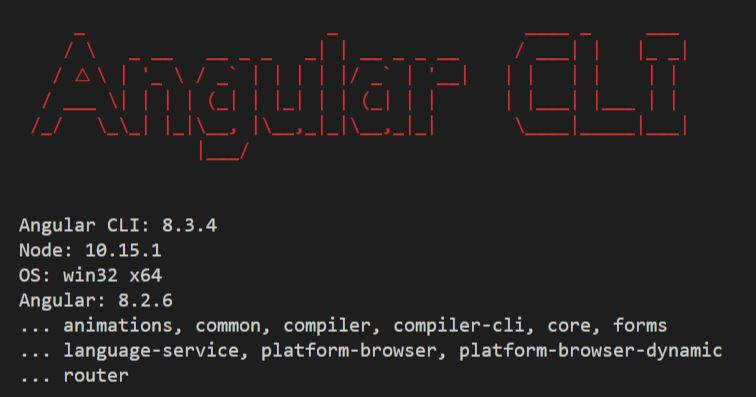
\includegraphics[width=0.65\textwidth]{images/angularversion}
    \caption{Versión Angular Cli}
    \end{figure}
    
    \FloatBarrier
    
    Una vez instalada la herramienta de comandos \textit{Angular Cli}, procedemos a crear nuestro proyecto base Angular ejecutando el comando \texttt{ng new estudio-medico-tfg2019}, generando un proyecto completo Angular junto con toda su estructura de carpetas.
    
    
    
    \subsection{Arquitectura de la aplicación Java Spring}
    
    
    \section{BackEnd}
    \subsection{Generación Proyecto Java Spring}
    \subsection{Arquitectura de la aplicación Angular}